\section{Utente Autenticato}

Di seguito vengono elencati i casi d'uso per l'utente autenticato.

\subsubsection{UC-U8}

    \begin{figure}[H]
      \begin{center}
        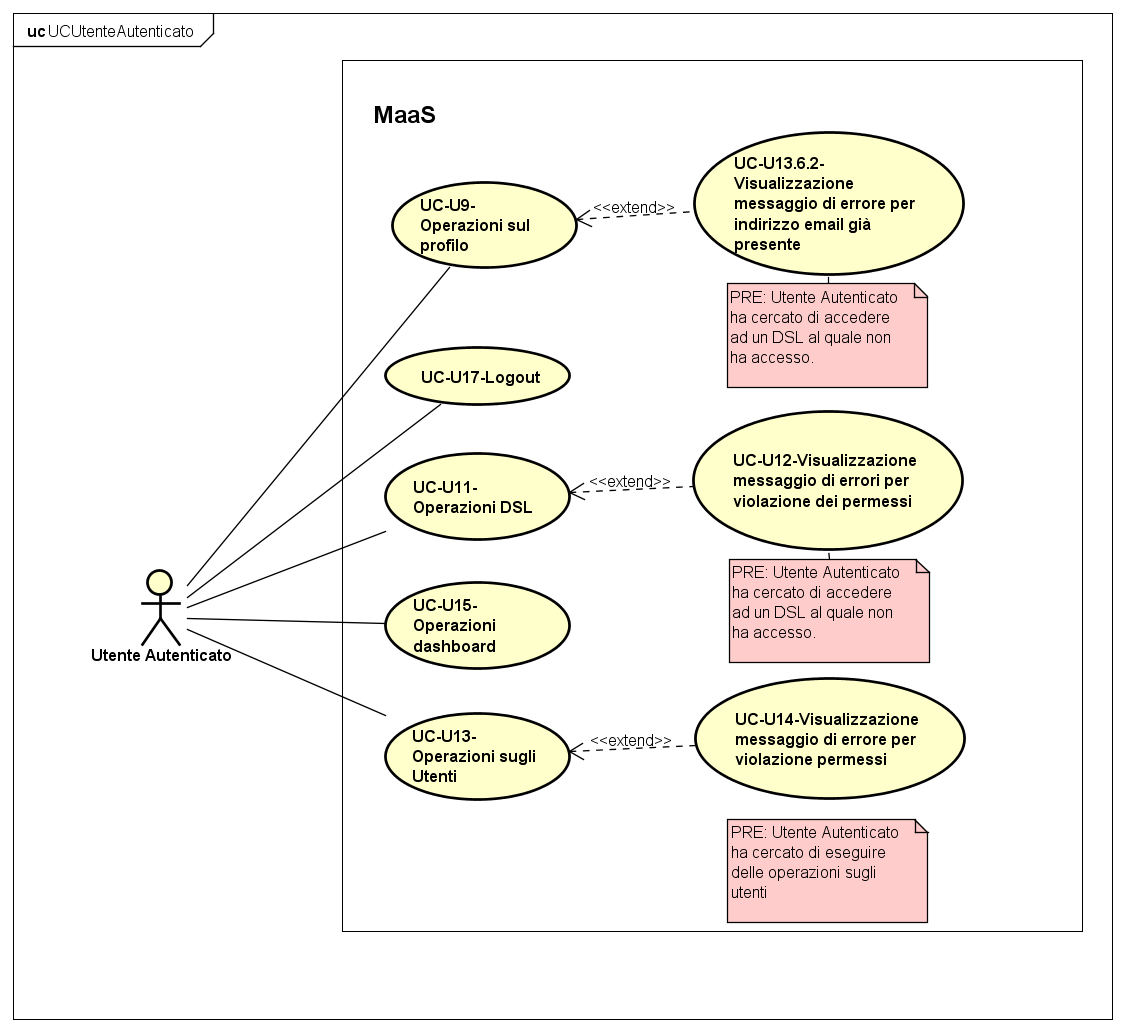
\includegraphics[width=12cm]{res/img/UCUtenti/UCUtenteA/UC-U8-OperazioniUtenteAutenticato}
      \caption{UC-U8 - Operazioni dell'utente autenticato}
      \end{center} 
    \end{figure}    
    
    %Tabella 
    \begin{center}
      \bgroup
      \def\arraystretch{1.8}     
      \begin{longtable}{  p{3.5cm} | p{8cm} } 
        
        \hline
        \multicolumn{2}{ | c | }{ \cellcolor[gray]{0.9} \textbf{UC-U8 - Operazioni dell'utente autenticato}} \\ 
        \hline
        
        \textbf{Attori Primari} & Utente autenticato \\ 
        \textbf{Scopo e Descrizione} & L’utente autenticato può: modificare il proprio profilo, effettuare delle operazioni nella pagina Dashboard, effettuare delle operazioni di creazione/modifica/esecuzione del DSL (a seconda dei suoi permessi) e gestire altri utenti (quest'ultima funzionalità è riservata ad un ruolo superiore o uguale all'admin). \\ 
        
        \textbf{Precondizioni}  & L’applicazione Maas è funzionante e pronta all'uso. L'utente autenticato può accedere alla propria pagina Dashboard. \\ 
        
        \textbf{Postcondizioni} & L'applicazione ha eseguito le azioni richieste dall'utente. \\ 
        \textbf{Flusso Principale} & 1. L'utente modifica il proprio profilo (UC-U9)
        
2. L'utente effettua delle operazioni nella pagina Dashboard (UC-U15)

3. L'utente effettua delle operazioni di creazione/modifica/esecuzione del DSL (a seconda dei suoi permessi) (UC-U11)

4. L'utente gestisce altri utenti (quest'ultima funzionalità è riservata ad un ruolo superiore o uguale all'admin) (UC-U13) \\
        \textbf{Estensioni} & 1. L'utente autenticato visualizza un messaggio di errore nella proceduro di modifica del profilo dovuto all'inserimento di un indirizzo email già presente (UC-U13.6.2)
        
2. L'utente autenticato visualizza un messaggio di errore durante le operazioni effettuate sul DSL dovuto alla violazione dei permessi (UC-U12)

3. L'utente autenticato visualizza un messaggio di errore durante le operazioni sugli utenti dovute alla violazione dei permessi (UC-u14) \\
        \textbf{Inclusioni} & Nessuna \\
      \end{longtable}
      \egroup
    \end{center} 


\subsubsection{UC-U9}

    \begin{figure}[H]
      \begin{center}
        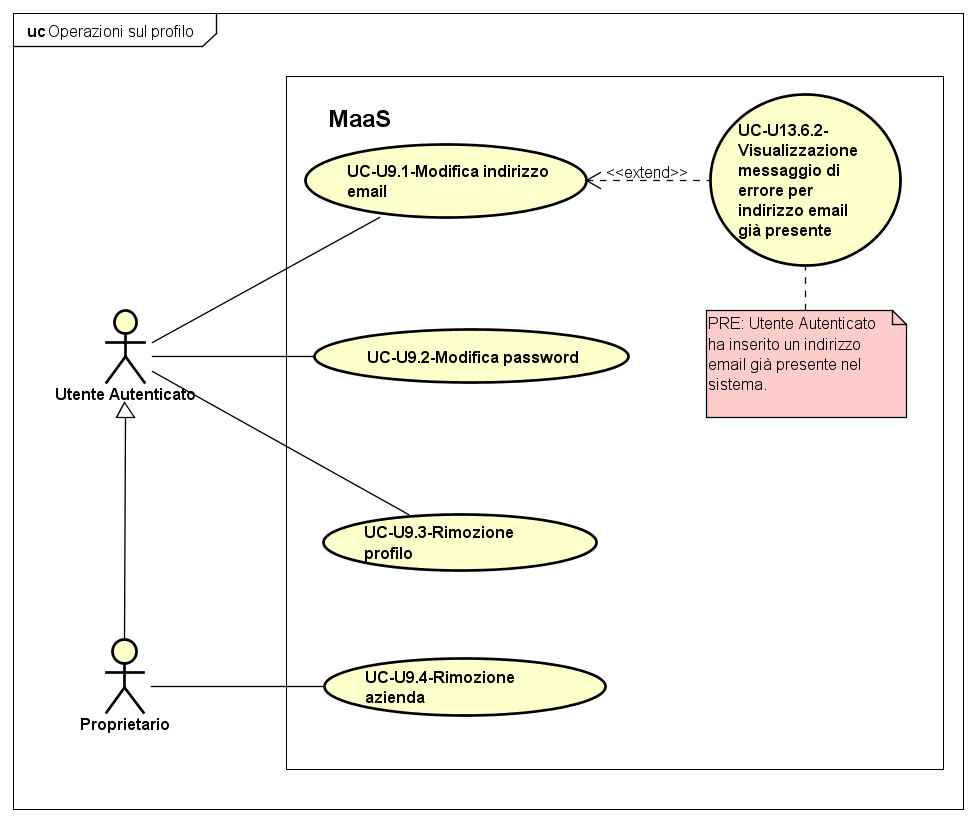
\includegraphics[width=12cm]{res/img/UCUtenti/UCUtenteA/UC-U9- Operazioni sul profilo/Operazioni sul profilo}
      \caption{UC-U9 - Operazioni sul profilo}
      \end{center} 
    \end{figure}    
    
    %Tabella 
    \begin{center}
      \bgroup
      \def\arraystretch{1.8}     
      \begin{longtable}{  p{3.5cm} | p{8cm} } 
        
        \hline
        \multicolumn{2}{ | c | }{ \cellcolor[gray]{0.9} \textbf{UC-U9 - Operazioni sul profilo}} \\ 
        \hline
        
        \textbf{Attori Primari} & Utente autenticato \\ 
        \textbf{Scopo e Descrizione} & L'utente autenticato visualizza la pagina per apportare modifiche al profilo personale. Può decidere di: modificare l'indirizzo email, la password, o rimuovere il profilo. \\ 
        
        \textbf{Precondizioni}  & L’applicazione Maas è funzionante e pronta all'uso. L'utente autenticato può accedere alla propria pagina Dashboard. \\ 
        
        \textbf{Postcondizioni} & Le (eventuali) modifiche del profilo richieste dall'utente sono state apportate. \\ 
        \textbf{Flusso Principale} & 1. L'utente modifica il proprio indirizzo email (UC-U9.1)
        
2. L'utente modifica la propria password (UC-U9.2)

3. L'utente rimuove il suo profilo/account (UC-U9.3)

4. Il proprietario rimuove la propria azienda (UC-U9.4) \\
        \textbf{Estensioni} & 1. L'utente visualizza un messaggio di errore durante la modifica dell'email dovuto all'inserimento di un indirizzo email già presente. \\
        \textbf{Inclusioni} & Nessuna \\
      \end{longtable}
      \egroup
    \end{center} 

    